\documentclass[12pt]{article}
\usepackage[utf8]{vietnam}
% Gói chèn ảnh
\usepackage{graphicx}
% Chèn hình lấn chữ
\usepackage{wrapfig}
% Văn bản mẫu
\usepackage{blindtext}
% Gói hộp văn bản \pbox
\usepackage{pbox}
% Gói xoay hộp
\usepackage{rotating}

\begin{document}

%\includegraphics[<option>]{<link>}
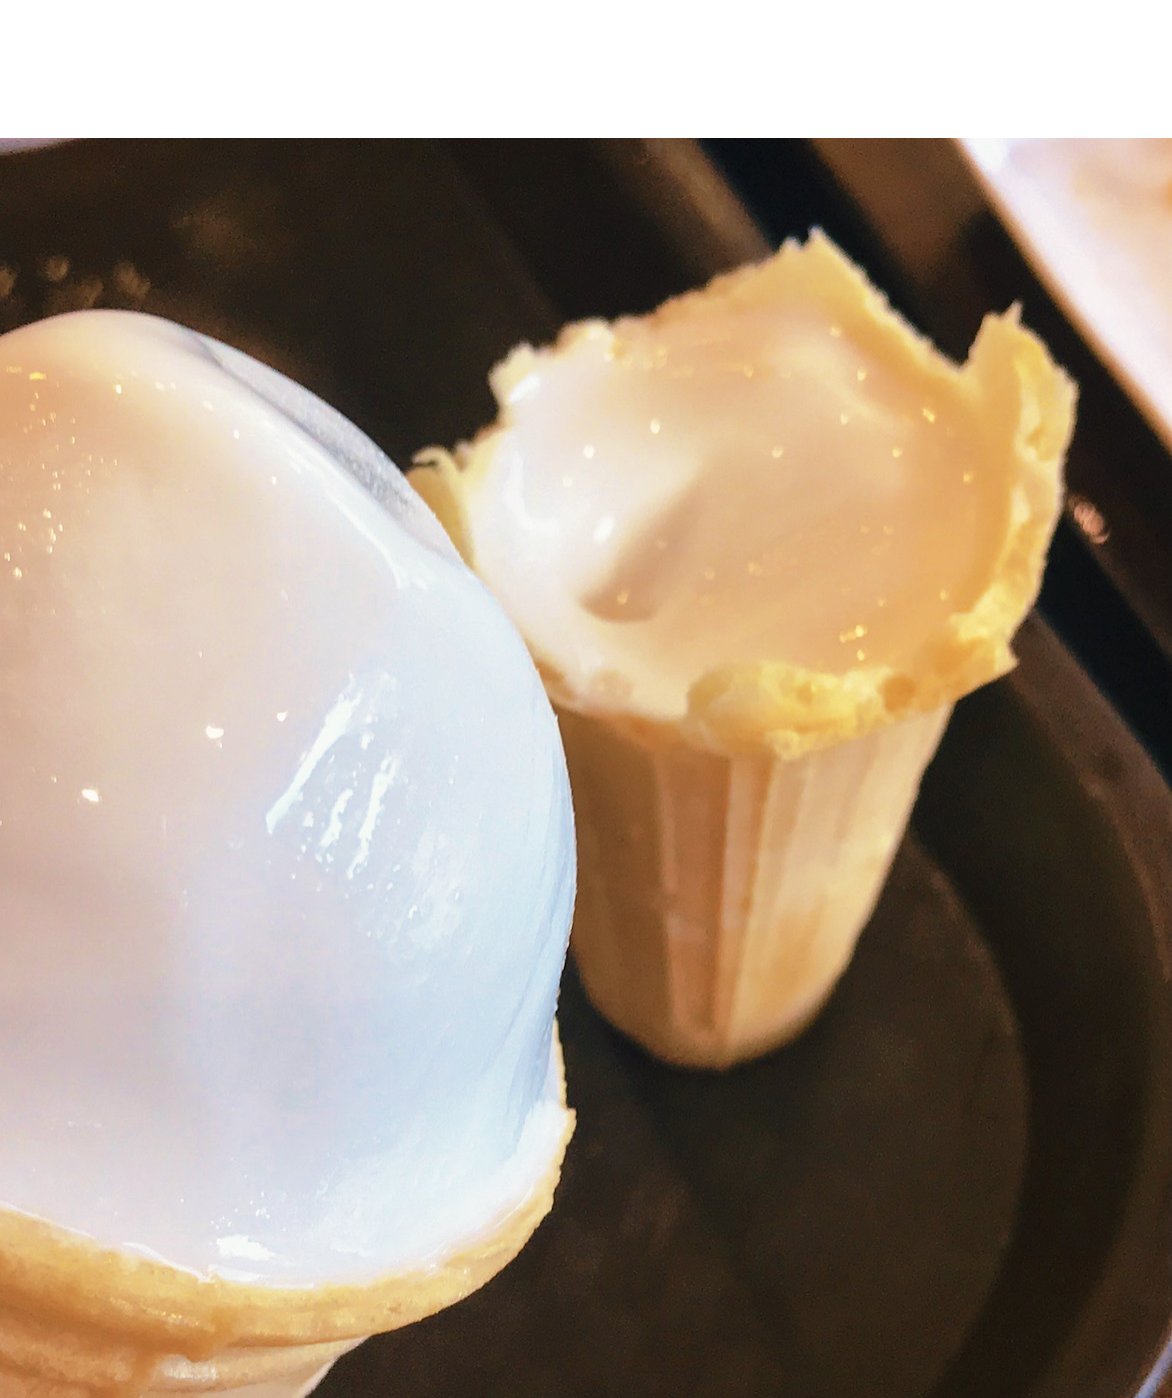
\includegraphics[scale=0.1]{cute.png}

% Môi trường figure
\begin{figure}[h!]
	\centering
	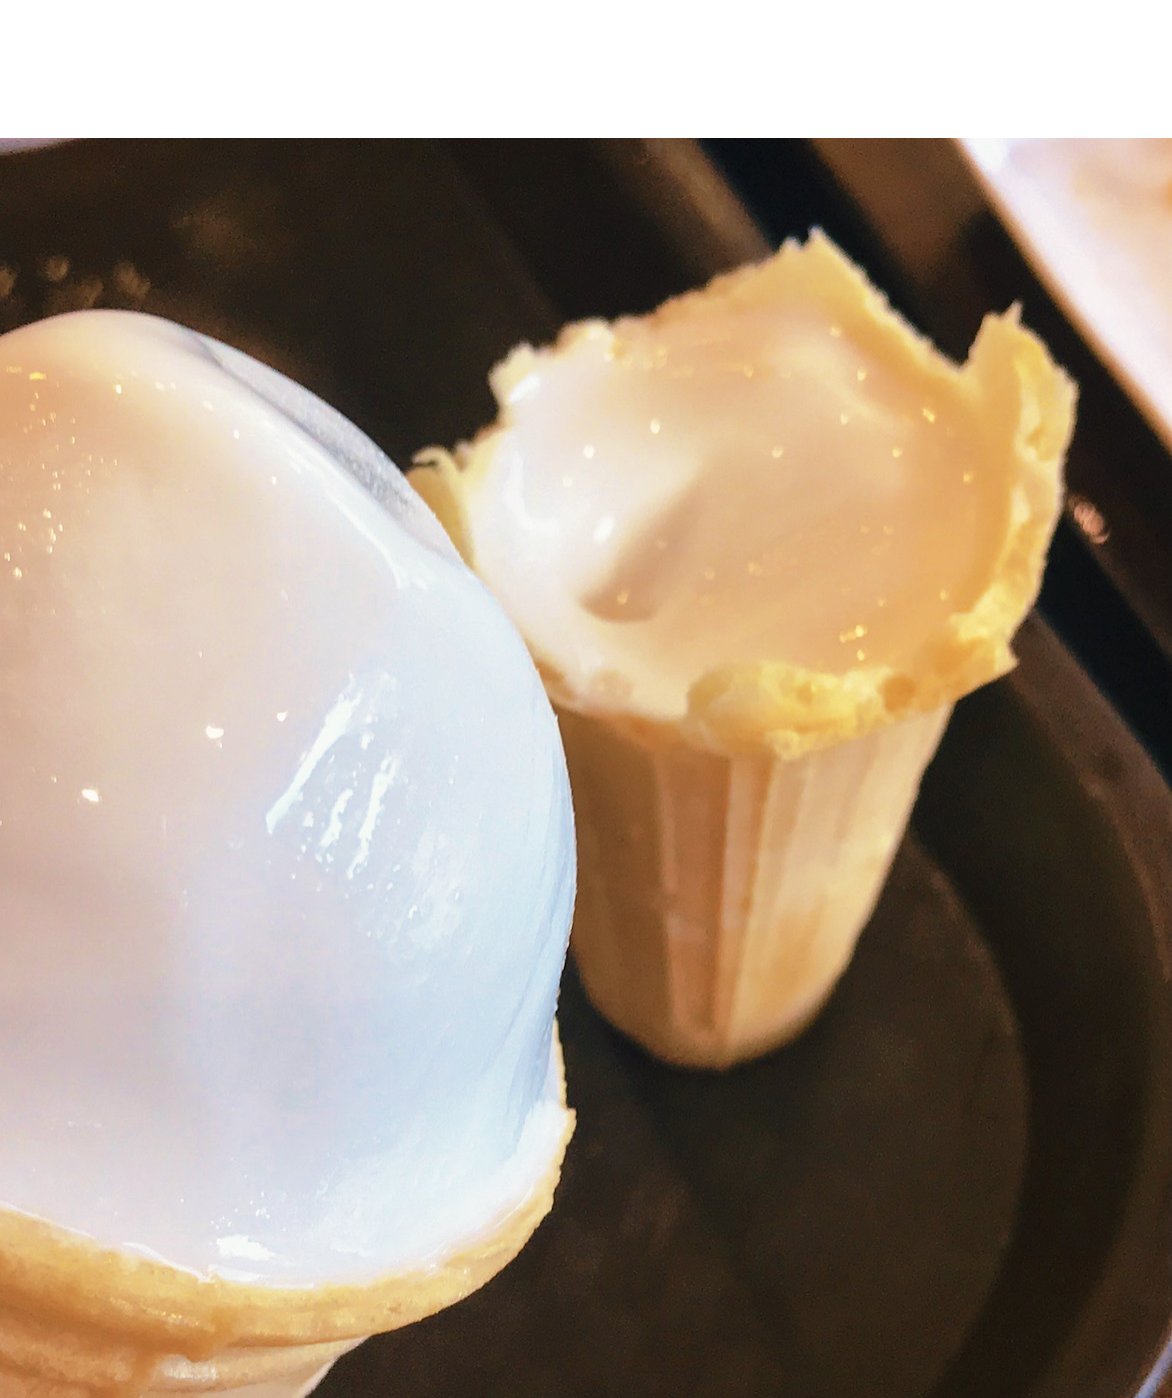
\includegraphics[scale=0.5]{cute.png}
	\caption{Cute lover}
	\label{fig:cute}
\end{figure}

\newpage

% [<number of line>]{<position>}
\begin{wrapfigure}[12]{h}{5cm}
    \centering
    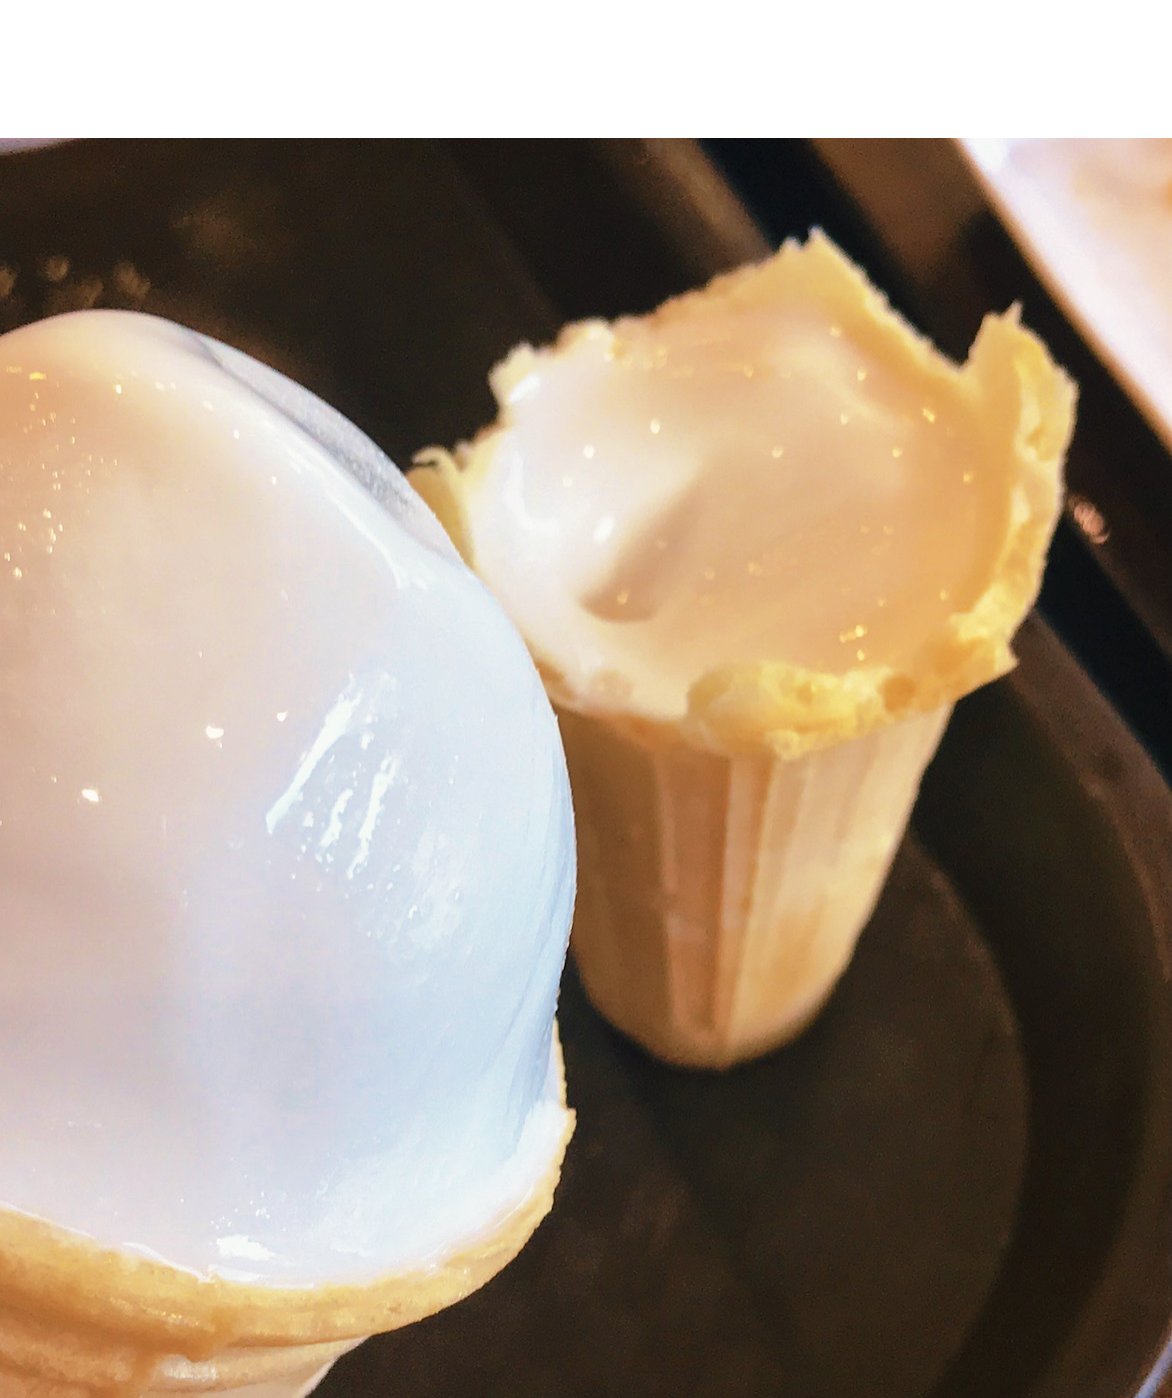
\includegraphics[scale=0.15]{cute.png}
    \caption{Cute Lover}
\end{wrapfigure}
\blindtext

% \parbox[<position>][<height>][<align>][<width>]{<text>}
a \parbox{5cm}{hộp văn bản gdg} a\\

\newpage

% Tạo ra Column paragraph
\begin{minipage}{0.3\textwidth}
	\blindtext
\end{minipage}
\quad
\begin{minipage}{0.3\textwidth}
	\blindtext
\end{minipage}
\quad
\begin{minipage}{0.3\textwidth}
	\blindtext
\end{minipage}

% Tạo hộp một dòng
% \makebox
%\mbox

%TẠO HỘP SỬ DỤNG LẠI
% Khởi tạo dòng lệnh \<tên lệnh>
\newsavebox{\boxname}
% Lưu nội dung vào lệnh
\savebox{\boxname}{$5^3$}
% Sử dụng lệnh
\usebox{\boxname}
\usebox{\boxname}
\usebox{\boxname}

% \framebox[<width>][<align>]{<text>}
a \framebox[5cm][c]{framebox} aa

% fbox[<text>]
a \fbox{fbox} a

hộp \raisebox{2pt}{raisebox}

% Hộp văn bản có thể kéo dãn, thay đổi kích thướcthước
% \resizebox{[horizontal space]}{<vertical space>}{<text>}
\resizebox{3cm}{1cm}{resizebox}

%\scalebox{<scale>}{<text>}
\scalebox{3}{s}

% Xoay hộp, sử dụng gói roating và môi trường rotate hoặc turn nhưng rotate không để lại khoảng trắng thừa
\vspace{3cm}
\begin{rotate}{90}
	Rotate
\end{rotate}
\end{document}